\documentclass[a4paper,10pt]{article}
\usepackage[margin=1in]{geometry}
\usepackage{polski}
\usepackage[utf8x]{inputenc}
\usepackage[unicode]{hyperref}
\usepackage{amssymb}
\usepackage{xifthen}
\usepackage[fleqn]{amsmath}
\usepackage{todonotes}
\usepackage{graphicx}
\usepackage{float}
\usepackage{fullpage}
\usepackage{epstopdf}
\usepackage{multirow}
\usepackage{subfig}
\usepackage[europeanresistors,americaninductors]{circuitikz}
\usetikzlibrary{patterns}
\newcommand{\withtodo}{0}

\def\arraystretch{1.2}

\begin{document}

\begin{table}
  \centering
  \def\arraystretch{1.5}
    \begin{tabular}{|l|l|l|l|} \hline
    Wydział:           & \multicolumn{2}{l|}{Dzień:Poniedziałek 14-17}    &Zespół:  \\
    Fizyki             &    \multicolumn{2}{l|}{Data: 13.03.2017}         &8             \\\hline
    Imiona i nazwiska: &Ocena z przygotowania:  &Ocena ze sprawozdania:   &Ocena końcowa: \\
    Marta Pogorzelska  &                        &                         &                \\
    Paulina Marikin    &                        &                         &\\\hline
    \multicolumn{2}{|l|}{Prowadzący:                 } &\multicolumn{2}{l|}{Podpis:             }  \\\hline
  \end{tabular}
\end{table}

\title{Ćwiczenie 27:\\Badanie właściwości statystycznych elektronów emitowanych z katody lampy próżniowej.}
\date{}
\maketitle{}

\section{Cel badań}
Zapoznanie się  z założeniami rozkładu Maxwella dla gazu doskonałego oraz sprawdzić poprawność zastosowania jej do opisu zbioru elektronów termicznych....

\section{Wstęp teoretyczny}
Rozkład Maxwella zakłada, że cząsteczki powietrza, a dokładniej gazu doskonałego, nie poruszają się z taką samą prędkością, tylko ich  wartości są różne i zawierają się w pewnym przedziale prędkości $<v, v + dv>$. Liczba cząstek, których prędkości zawierają się w tych granicach na jednostkę objętości, wynosi:

\begin{equation}
n(v) = 4\pi Nv^2(\frac{a}{\pi})^{\frac{3}{2}}exp(-av^2)
\end{equation}
,gdzie  $N$ - ogólna liczba cząstek na daną objętość, $v$ - prędkość cząsteczki, $a = \frac{m}{2kT}$, m - masa cząsteczki, $k$ – stała Boltzmanna, $T$ – temperatura wyrażona w Kelwinach.
\vspace{0,4cm}

Według powyższego założenia zamiast mówić o prędkości pojedynczych cząsteczek gazu, mówimy o rozkładzie prędkości tych cząsteczek. Statystyka Maxwella pokazuje również, że prędkości tych cząsteczek oraz ich rozkład zależą  od temperatury. Wraz ze wzrostem temperatury rozkład poszerza się i spłaszcza a prędkości cząsteczek zwiększają się.

Opisany powyżej rozkład można zastosować  do opisu zbioru elektronów termicznych emitowanych przez katodę lampy elektronowej. Wynika to ze zjawiska termoemisji oraz przybliżenia gazu elektronowego do gazu doskonałego. Podstawą do takich założeń, jest między innymi fakt, że koncentracja elektronów, które opuściły metal jest znacząco mniejsza niż tych pozostałych w metalu. Pozwala to na zaniedbanie oddziaływań między tymi cząsteczkami. Elektrony $\gamma$, które pokonały siły wiążące je z metalem i wydostały się poza barierę potencjału na zewnątrz, posiadają energię kinetyczną $E \geq eU_a$, a ich liczba wyraża się wzorem:

\begin{equation}
\gamma (E) = N \sqrt{\frac{1}{2\pi kT}}exp(-\frac{E}{kT})
\end{equation}
,gdzie $T$ – temperatura lampy  próżniowej wyrażona w Kelwinach.
\vspace{0,4cm}

Rozkład prędkości elektronów termicznych można wyznaczyć między innymi na podstawie pomiarów prądu anodowego w funkcji napięcia hamującego, co zostanie wykorzystane w tym doświadczeniu.

Zależność między prądem anodowym $I_a$ i napięciem $U_a$ można zapisać wzorem:

\begin{equation}
  I_a(U_a) = I_{a0}\exp{\Big(\frac{-eU_a}{kT}\Big)}
\end{equation}

gdzie $I_{a0}$ – prąd anodowy przy napięciu $U_a = 0$,  $e$ - ładunek elementarny.


\section{Metoda przeprowadzenia badań i pomiarów, materiały, aparatura}

\begin{figure}[H]
\centering
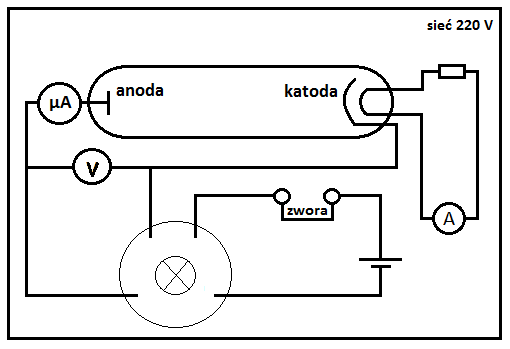
\includegraphics[width=0.5\textwidth]{schemat.png}
\end{figure}

Najpierw należało połączyć elementy układu według schematu przedstawionego powyżej. Po dokładnym sprawdzeniu podłączenia układu przyrządy zostały włączone. Następnie ustawiony został prąd żarzenia lampy elektronowej wyznaczony przez prowadzącego. Po odczekaniu kilku minut i ustaleniu się wartości prądu żarzenia wykonano pomiary wartości prądu anodowego w zależności od napięć między katodą i anodą. Wykonano dwie serie dla dwóch różnych wartości prądu żarzenia pamiętając, aby wartości pomiarów prądu anodowego nie spadły poniżej $\frac{1}{3}$ początkowej wartości. Po każdej serii, przy zmianie prądu żarzenia, odczekano kilka minut w celu ustabilizowania się jego wartości.

\hspace{2in}

Aparatura pomiarowa
\begin{itemize}
  \item Woltomierz cyfrowy klasy 0,3\%
  \item Amperomierz analogowy klasy 1,5\%
  \item Amperomierz cyfrowy klasy 0,3\%
\end{itemize}

\hspace{2in}

Pozostałe elementy
\begin{itemize}
  \item Kable
  \item Lampa próżniowa
  \item Dzielnik napięcia
\end{itemize}

\section{Wyniki pomiarów}

\begin{tabular}{|l|r|r|r|r|}
\hline
&\multicolumn{2}{c|}{Seria 1} &\multicolumn{2}{c|}{Seria 2}\\\hline
 &\multicolumn{2}{c|}{$I_ż$ = 0.448(2)A} &\multicolumn{2}{c|}{$I_ż$ = 0.528(3)A}\\\hline
&  $U_a$[mV] &  $I_a$[$\mu A$] &  $U_a$[mV] &  $I_a$[$\mu A$] \\\hline
0  &     -0.0(1) &        15 &     -0.7(1) &       150 \\\hline
1  &    -10.2(1) &        14 &    -14.3(1) &       140 \\\hline
2  &    -16.9(2) &        13 &    -30.2(2) &       130 \\\hline
3  &    -24.9(2) &        12 &    -47.2(2) &       120 \\\hline
4  &    -32.9(2) &        11 &    -63.5(3) &       110 \\\hline
5  &    -42.4(2) &        10 &    -79.5(3) &       100 \\\hline
6  &    -51.9(3) &         9 &    -98.3(4) &        90 \\\hline
7  &    -63.7(3) &         8 &   -116.5(4) &        80 \\\hline
8  &    -75.0(3) &         7 &   -136.4(5) &        70 \\\hline
9  &    -89.3(4) &         6 &   -157.8(6) &        60 \\\hline
10 &   -104.6(4) &         5 &   -181.2(6) &        50 \\\hline
\end{tabular}

\section{Analiza pomiarów niepewności}
\begin{center}
\begin{tabular}{|c c|}
  \hline
  $\ln{\frac{I_a}{I_{a0}}}$& niepewność \\
  \hline
   0.00  &0.02  \\\hline
  -0.069 &0.022 \\\hline
  -0.143 &0.023 \\\hline
  -0.223 &0.024 \\\hline
  -0.31  &0.03  \\\hline
  -0.41  &0.03  \\\hline
  -0.51  &0.03\\\hline
  -0.63  &0.03\\\hline
  -0.76  &0.04\\\hline
  -0.92  &0.04\\\hline
  -1.09  &0.05\\\hline
\end{tabular}
\end{center}

\vspace{1cm}
Niepewność logarytmu została policzona metodą propagacji niepewnosci przy użyciu wzoru:

\begin{equation}
u(ln{\frac{I_a}{I_{a0}}}) = \sqrt{(\frac{1}{I_a} u(I_a))^2 + (-\frac{1}{I_{a0}} u(I_{a0})^2}
\end{equation}

W celu sprawdzenia poprawności postawionej na początku tezy, zlogarytmowano obie strony równania (3), a następnie wykreślono dla tych  zależności dla obu serii pomiarowych wykresy (które powinny przedstawić zależność liniową) i dopasowano do nich proste jednoparametrowe ($y=ax$) przy użyciu funkcji \emph{curvefit} biblioteki \emph{scipy.optimize} w Pythonie. Obliczono również niepewnosci pomiarów pochodzące od użytych przyrządów. Dla amperomierza analogowego, którym wykonywane były pomiary,  niepewność wyliczono ze wzoru:

\begin{equation}
u(I) = \sqrt{(\frac{\Delta I}{\sqrt{3}})^2 + (\frac{\Delta I_e}{\sqrt{3}})^2}
\end{equation}

,gdzie $\Delta I = \frac{klasa*zakres}{100}$, $\Delta I_e = \frac{zakres}{podziałka}$ - niepewnosć eksperymentatora, klasa = 1,5\%, zakres wynosił kolejno 25 $\mu$A dla pierwszej i 0,15 mA dla drugiej serii pomiarowej.

\vspace{0,4cm}
Natomiast dla woltomierza cyfrowego niepewnosć wyliczono ze wzoru:

\begin{equation}
u(U) = \frac{\Delta U}{\sqrt{3}}
\end{equation}

,gdzie $\Delta$ U = klasa * rdg + 1dgt, klasa = 0,3\%, 1dgt = 1mV.

\begin{figure}[H]
\centering
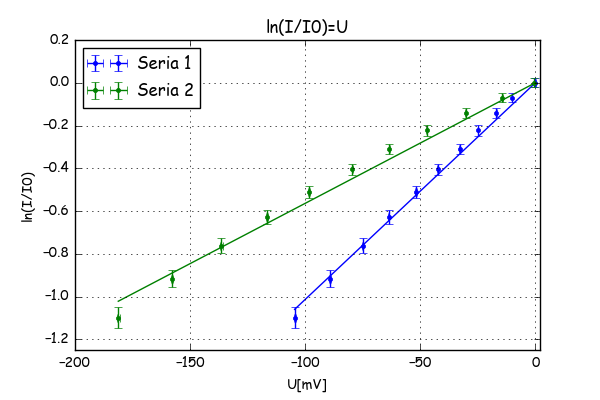
\includegraphics[width=0.9\textwidth]{zarzenie.png}
\caption{Wykresy nr 1: Zależność $ln{\frac{I}{I_0}}$ od napięcia hamującego U}
\end{figure}

\begin{itemize}
  \item Seria 1: $a = 0.01013(13)$
  \item Seria 2: $a = 0.00563(12)$
\end{itemize}

Niepewność wyznaczenia prądu wyliczona ze wzoru (3) dla obu serii pomiarowych wyniosła odpowiednio $0.25\mu$A i $2.25\mu$A.

Zgodnie z postawioną teorią współczynnik proporcjonalnoci $a = \frac{-e}{kT}$. Przekształcając wzór można więc wyznaczyć temperaturę lampy próżniowej $T = \frac{-e}{ka}$. Jej niepewnosć została  policzona natomiast ze wzoru:

\begin{equation}
u(T) = \sqrt{(\frac{\partial T}{\partial a} u(a))^2 } = -\frac{e}{ka^2} u(a)
\end{equation}

Tak wyliczona temperatura lampy prożniowej wraz niepewnosciami dla obu serii pomiarowych wynosi:

\begin{itemize}
  \item $T_1 = 1145(15)$K
  \item $T_2 = 2057(43)$K
\end{itemize}

\begin{figure}[H]
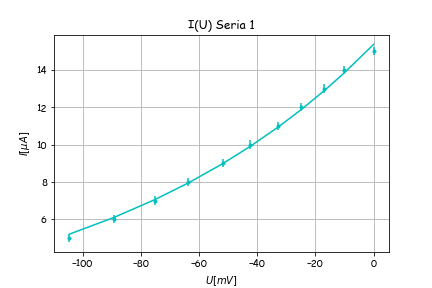
\includegraphics[width=0.5\textwidth]{zarzenieU1.png}
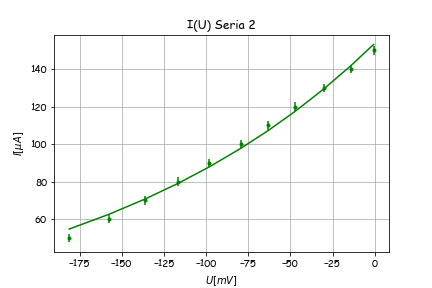
\includegraphics[width=0.5\textwidth]{zarzenieU2.png}
\caption{Wykresy nr 2 i 3: Zależność $I(U)$ dla obu serii pomiarowych}
\end{figure}

Porównując wykresy (2) i (3) do zależność wzoru (2) można zauważyć, że wykres funkcji (2) zależny jest przede wszystkim od energii i rośnie do $\infty$ wraz z jej spadkiem. Napięcie zależne jest od energii w sposób liniowy: $E \geq eU_a$, zatem im mniejsze napięcie  tym wykresy funkcji (2) i (3) również powinny zbliżać się do $\infty$. Wykreślone wykresy w tym doświadczeniu przedstawiają taką zależność.

\begin{figure}[H]
 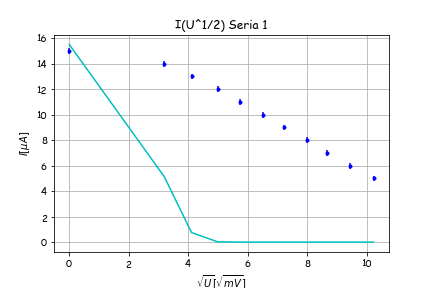
\includegraphics[width=0.5\textwidth]{zarzenieU12.png}
 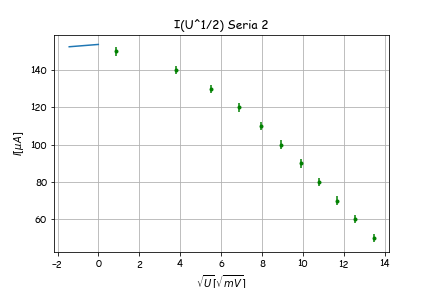
\includegraphics[width=0.5\textwidth]{zarzenieU22.png}
 \caption{Wykresy nr 4 i 5: Zależność $I(U^{\frac{1}{2}})$ dla obu serii pomiarowych}
 \end{figure}

Porównując wykresy (4) i (5) do zależność wzoru (1) można zauważyć, że wykres funkcji (1) zależny jest przede wszystkim od prędkości cząsteczek. Początkowo wykres wzrasta a następnie maleje i zbliża się do 0 wraz ze wzrostem prędkości. Napięcie związane jest z prędkością zależnością: $v = \sqrt{\frac{2eU_a}{m}}$, zatem im wyższe napięcie  tym wykresy funkcji (4) i (5) również powinny zbliżać się do 0. Wykreślone wykresy w tym doświadczeniu przedstawiają taką zależność i dążą do 0, jednakże nie można zaobserwować początkowego wzrostu. Wynikać to może z niewystarczającej liczby wykonanych w tym badaniu pomiarów.

\section{Wnioski}
 Na podstawie wykonanych pomiarów oraz przeanalizowania danych doświadczalnych i wykreślonych na ich podstawie wykresów można potwierdzić wstępne założenia o poprawności zastosowania rozkładu Maxwella dla elektronów termicznych. Wykres zależności wartości logarytmu naturalnego unormowanego prądu anodowego $\frac{I_a}{I_{a0}}$ od napięcia $U_a$ przedstawia zależność liniową co skłania ku potwierdzeniu tezy. Zależność wykresów (4) i (5) jest zbliżona do teorii, a niedokładność można byłoby zweryfikować i ewentualnie wyeliminować wykonując kolejne serie pomiarów z większą częstotliwością wykonywanych pomiarów i przeprowadzając badanie z większą dokładnością.
 \end{document}
